\subsubsection{Szczegóły budowania zbioru balancing}

Znalezienie zbioru balancing jest trudniejsze, z racji na dodatkowe obostrzenia związane z jego rozmiarem oraz wartością
helpfulness.
Zbiór $\bar{S}$ musi mieć ten sam rozmiar co zbiór $S$ oraz jego wartość helpfuless musi być tak duża jak to możliwe,
lecz nie mniejsza niż $-k+1$-helpful, jeśli $S$ był $k$-helpful.
Idea budowania zbioru balancing polega na rozpoczęciu od pustego zbioru $\bar{S}$ i wybraniu podzbioru
ze zbioru BIG SET, który zwiększy jego rozmiar tak bardzo jak to możliwe oraz jednocześnie zmniejszy jego wartość
helpfulness tak mało jak to możliwe.
Algorytm podzielony jest na trzy fazy.
Pierwsza faza dodaje do zbioru wierzchołki, których wartości helpfulness są $\geq$ $0$.
Druga faza próbuje znaleźć podzbiory wierzchołków, które dodane do $\bar{S}$, pozostawią jego helpfulness na jednym
poziomie - szuka zbiorów $0$-helpful.
Każda z tych faz kończy swoje wywołanie jeśli $\bar{S}$ jest wystarczająco duży.
Jeśli dwie pierwsze fazy są niewystarczające, uruchamiana jest trzecia faza, która oparta jest na zachłannym dobieraniu
wierzchołków, w celu dokończenia budowania zbioru balancing.

\begin{figure}[h]
\begin{subfigure}{.32\textwidth}
    \centering
    \fbox{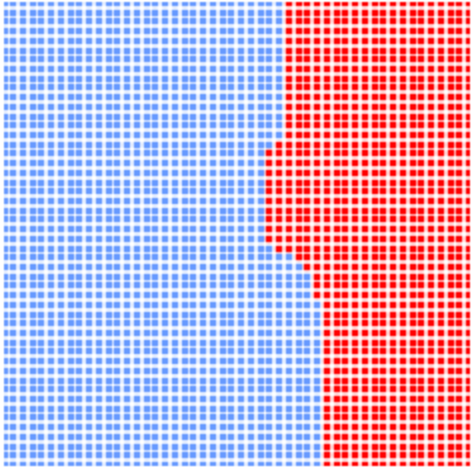
\includegraphics[width=0.7\textwidth]{images/helpful-balancing/3}}
    \caption[short]{podział}
\end{subfigure}
\begin{subfigure}{.32\textwidth}
    \centering
    \fbox{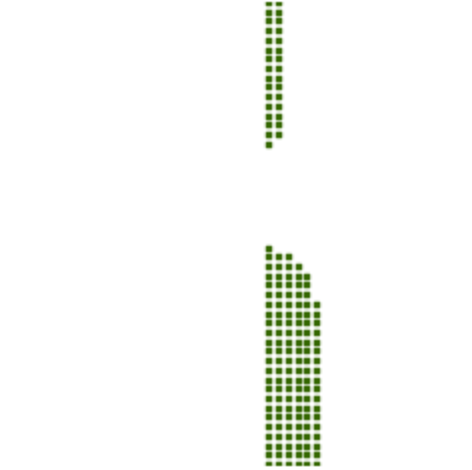
\includegraphics[width=0.7\textwidth]{images/helpful-balancing/6}}
    \caption[short]{faza 1}
\end{subfigure}
\begin{subfigure}{.32\textwidth}
    \centering
    \fbox{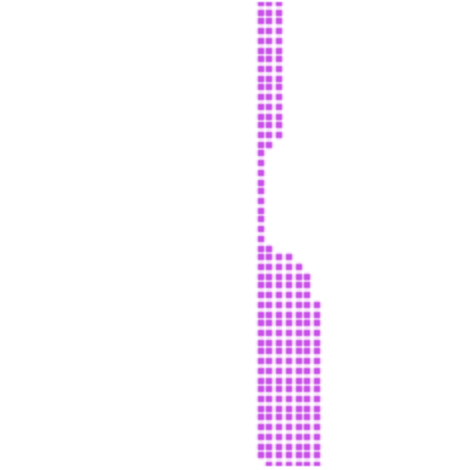
\includegraphics[width=0.7\textwidth]{images/helpful-balancing/4}}
    \caption[short]{faza 2}
\end{subfigure}
\caption{Obrazki przedstawiają fazę pierwszą oraz fazę drugą budowania zbioru balancing.
Ten sam przypadek podziału można znaleźć na rysunku \ref{im:balancing}.}
\label{im:balancing:details}
\end{figure}

\textbf{Faza 1}

Pierwsza faza jest najmniej skomplikowana.
Dopóki w zbiorze BIG SET są wierzchołki z wartościami helpfulness $\geq$ $0$, wierzchołek z największą wartością
helpfulness dodawany jest do zbioru $\bar{S}$.
Te wierzchołki uznawane są jako wierzchołki, które należą już do drugiej partycji, więc wartości helpfulness
ich sąsiadów z poprzedniej partycji muszą wzrosnąć o 2.
Podczas tej fazy wielkość $\bar{S}$ wzrasta, a wartość $H(\bar{S})$ pozostaje taka sama lub się powiększa.
Faza pierwsza kończy się jeśli utworzony zostanie zakładany zbiór balancing lub nie ma więcej wierzchołków
w zbiorze BIG SET, których wartości helpfulness są przynajmniej równe $0$.

\vspace{8mm}
\textbf{Faza 2}

Ta faza próbuje znaleźć zbiory $0$-helpful, to znaczy podzbiory zbioru BIG SET, które przeniesione do $\bar{S}$,
nie zmniejszą jego wartości helpfulness.
Koncepcja tej fazy polega na przeprowadzeniu kilku wyszukiwań, rozpoczynając od pojedynczego wierzchołka
$-1$-helpful lub $-2$-helpful.
Każde z wyszukiwań próbuje dopełnić swój podzbiór wierzchołków do zbioru $0$-helpful.
Ważną obserwacją jest, że na początku tego etapu BIG SET nie zawiera żadnych wierzchołków z wartością
helpfulness większą bądź równą zero.

\begin{figure}[h]
    \centering
    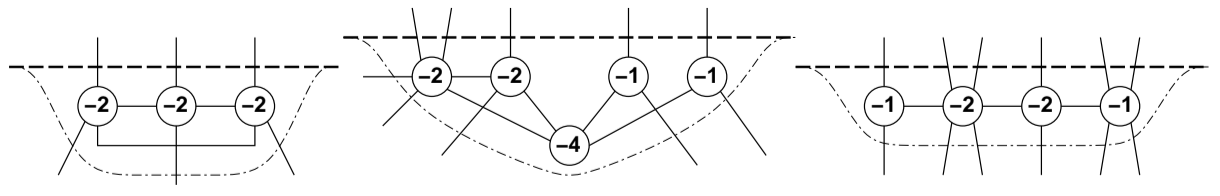
\includegraphics[width=0.95\linewidth]{images/0-helpful-sets}
    \caption{Przykłady zbiorów 0-helpful. Źródło: \cite{article}.}
    \label{im:0-helpful}
\end{figure}

Rysunek \ref{im:0-helpful} pokazuje przykładowe zbiory $0$-helpful.
Nie ma jednego przepisu na zbiór $0$-helpful, mogą być to różne konstrukcje wierzchołków, a intencją drugiej fazy
jest znalezienie jak największej liczby tego typu zbiorów.

Rysunek \ref{im:phase_2} pokazuje drugą fazę.
Tak jak w fazie pierwszej, wykorzystywana jest ta sama metoda budowania zbioru (sekcja $4.1.6$).
Jednak zamiast przenosić wierzchołki bezpośrednio do $\bar{S}$, są one przechowywane w zbiorze o nazwie $-2$-SET.
$-2$-SET zawiera aktualny podzbiór wierzchołków, który faza druga próbuje dopełnić do zbioru $0$-helpful.
Niech $k' = k + H(\bar{S})$ będzie poprawą długości granicy, spowodowaną przez przeniesienie $S$ i $\bar{S}$, każdy
na odpowiednią stronę podziału.
Na początku każdego poszukiwania zbioru $-2$-SET rozpatrywane są jedynie wierzchołki z wartością helpfulness, wynoszącą
$max(-2, -k'+1)$.
Następnie tylko wierzchołki, które są przynajmniej $0$-helpful mogę być umieszczone w zbiorze $-2$-SET.
To gwarantuje, że dowolny $-2$-SET może zostać przeniesiony do $\bar{S}$ na każdym etapie algorytmu, bez znaczącego
zmniejszania jego wartości helpfulness.
Jest to szczególnie istotne jeśli $-2$-SET jest wystarczająco duży, aby zakończyć balansowanie.
Podsumowując:
\begin{itemize}
    \item {tylko wierzchołki $-1$-helpful oraz $-2$-helpful ze zbioru BIG SET są rozważane na początku budowania $-2$-SET,}
    \item wartość helpfulness zbioru $-2$-SET jest co najmniej równa $-2$ i nigdy nie maleje,
    \item jeśli $k'$ wynosi $2$ tylko wierzchołki $-1$-helpful mogą zostać wybrane oraz
    \item jeśli $k'$ wynosi $1$ faza druga w ogóle się nie rozpoczyna.
\end{itemize}

Jeśli wyszukiwanie zbioru $-2$-SET zakończy się i jego wartość helpfulness jest mniejsza od $0$ to jest przechowywany
do dalszego użycia.
\begin{figure}[h]
    \centering
    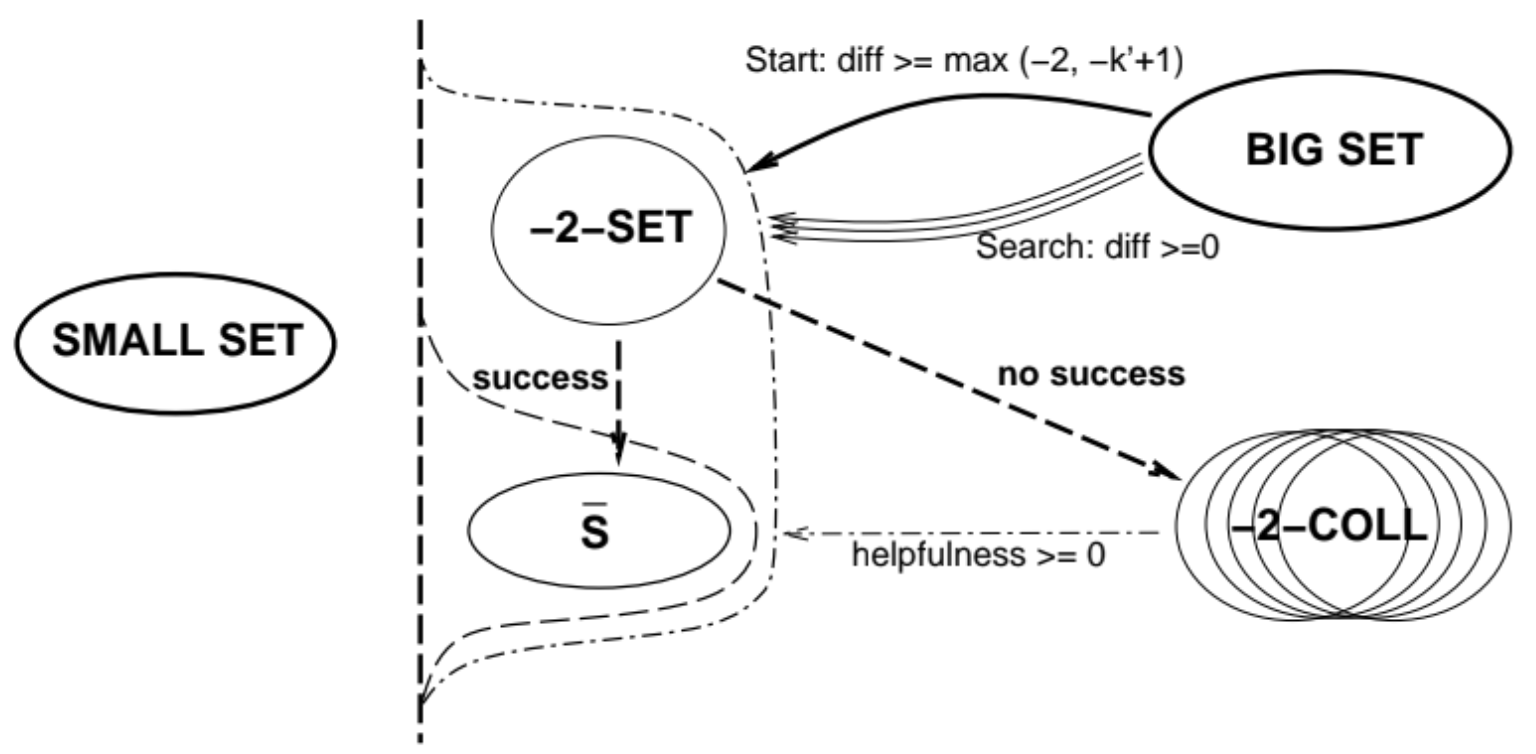
\includegraphics[width=0.65\linewidth]{images/phase2}
    \caption{Obrazek przedstawiający fazę 2. Źródło: \cite{article}.}
    \label{im:phase_2}
\end{figure}
\newpage

\begin{pseudocode}
@\underline{PROCEDURE Phase 2}@
  WHILE $(|\bar{S}| < |S|)$ AND BIG SET contains nodes with helpfulness $\geq$ $max(-2, -k + 1 - H(\bar{S})$
    start building a $-2$-SET with the max. helpful node;

    WHILE H$(-2$-SET$)$ $<$ $0$ AND $(|-2$-SET$|$ + $|\bar{S}|$ $<$ $|S|)$ AND
          BIG SET has node with helpfulness $\geq$ $0$
      move node with the highest helpfulness to $-2$-SET;
    ENDWHILE

    IF H$(-2$-SET$)$ $\geq$ 0
      move $-2$-SET to $\bar{S}$;
      WHILE $(|\bar{S}|$ $<$ $|S|)$ AND $-2$-COLL contains sets $S'$ with H$(S')$ $\geq$ $0$
        take set $S'$ $\in$ $-2$-COLL with max. helpfulness;
        IF $|S'|$ + $|\bar{S}|$ $<$ $|S|$
          move $S'$ to $\bar{S}$;
        ELSE
          reduce $S'$ to $|S|$ - $|\bar{S}|$ and move it to $|\bar{S}|$;
        ENDIF
    ELSE IF $| -2$-SET$|$ + $|\bar{S}|$ = $|S|$
      move $-2$-SET to $\bar{S}$;
    ELSE
      move $-2$-SET to $-2$-COLL;
    ENDIF
  ENDWHILE
\end{pseudocode}
\vspace{-8mm}
\captionof{listing}{Algorytm przedstawiający fazę drugą. Źródło: \cite{article}.}
\label{code:phase_2}
\vspace{4mm}
Kolekcja zbiorów $-2$-SET jest nazywana $-2$-COLL.
Zawiera ona podzbiory wierzchołków, które są co najmniej $-2$-helpful.
Wiele z nich może zostać zbiorami $0$-helpful, jeśli inne zbiory $-2$-SET zostaną przeniesione do $\bar{S}$.
Aktualizacja wartości helpfulness sąsiadów podczas budowania zbioru $-2$-SET następuje tylko dla wierzchołków,
które są częścią zbioru BIG SET.
Zbiory $-2$-SET będące w zbiorze $-2$-COLL nie są uznawane za zbiory, które zmieniły stronę partycjonowania.
W związku z tym, jeśli $-2$-SET nie może zostać uzupełniony wierzchołkami, aby być $0$-helpful i jest przenoszony
do zbioru $-2$-COLL, to wartości helpfulness wierzchołków w zbiorze BIG SET, które były jego sąsiadami, są przywracane
do poprzednich wartości.
Na tym etapie algorytmu podczas budowania zbioru $-2$-SET, wartości helpfulness sąsiednich wierzchołków w zbiorze
$-2$-COLL nie są zmieniane, ponieważ wierzchołki w zbiorze $-2$-COLL nie są brane pod uwagę przy budowaniu zbiorów
$-2$-SET.
Tylko jeśli zbiór $-2$-SET zostanie $0$-helpful i jest przenoszony do $\bar{S}$ to aktualizowane są wartości helpfulness
jego sąsiadów będących w zbiorze $-2$-COLL.

Algorytm \ref{code:phase_2} przedstawia fazę drugą.
Szukanie zbioru $-2$-SET kończy się w następujących przypadkach:
\begin{enumerate}
    \item {Wartość helpfulness zbioru $-2$-SET staje się większa bądź równa 0. W tym przypadku cały zbiór $-2$-SET
    przenoszony jest do zbioru $\bar{S}$. Wartości helpfulness sąsiednich wierzchołków znajdujących się w zbiorze
    $-2$-COLL są aktualizowane. Każda taka aktualizacja wartości helpfulness dla wierzchołka w zbiorze $-2$-COLL
    skutkuje tym, że wartość helpfulness jednego znajdującego się tam zbioru $-2$-SET podnosi się o 2. W związku z tym
    wiele z nich może zostać co najmniej $0$-helpful, a następnie zostać przeniesione do $\bar{S}$.
    Algorytm wybiera zawsze zbiór $-2$-SET z największą wartością helpfulness i przenosi go do $\bar{S}$, tak długo
    jak w $-2$-COLL są takie zbiory.

    Jeśli, któryś z tych zbiorów jest większy niż $|S| - |\bar{S}|$ to jest redukowany do odpowiedniego rozmiaru, poprzez
    usuwanie ostatnio dodanych elementów. Rezultatem takiej redukcji jest $|\bar{S}| = |S|$ oraz zakończenie
    wykonania procedury.}
    \item {Partycja osiąga odpowiedni rozmiar, to znaczy $|-2$-SET$|$ $+$ $|\bar{S}|$ $=$ $|S|$. W tym przypadku wartość
    helpfulness zbioru $-2$-SET wciąż wynosi co najmniej $max(-2, -k' + 1)$ (co jest zagwarantowane procesem jego budowania)
    i może on zostać przeniesiony do zbioru $\bar{S}$. Partycja osiąga w tym wypadku odpowiedni rozmiar i następuje
    zakończenie procedury.}
    \item {Nie ma więcej wierzchołków w zbiorze BIG SET z wartością helpfulness większą bądź równą $0$. W tym wypadku
    aktualnie budowany $-2$-SET nie może zostać powiększony o kolejne wierzchołki, w związku z tym jest przenoszony do
    zbioru $-2$-COLL, gdzie oczekuje na późniejsze wykorzystanie.}
\end{enumerate}

\vspace{8mm}
\textbf{Faza 3}

Ta faza wybiera wierzchołki ze zbioru BIG SET oraz zbiory $-2$-SET ze zbioru $-2$-COLL w celu przeniesienia do
$\bar{S}$.
Wybiera wierzchołek lub zbiór z największą wartością helpfulness tak długo, aż przeniesienie go nie obniży wartości
helpfulness zbioru $\bar{S}$ poniżej wartości $-k+1$.
Jeśli jakiś zbiór $-2$-SET ze zbioru $-2$-COLL jest użyteczny, ale jego rozmiar jest większy niż $|S| - |\bar{S}|$,
to jego rozmiar jest redukowany.
Faza $3$ kończy swoje wywołanie, jeśli przeniesienie jakiegokolwiek zbioru $-2$-SET lub wierzchołka, spowoduje
obniżenie wartości helpfulness zbioru $\bar{S}$ poniżej $-k+1$ lub jeśli uda się wypełnić zbiór $\bar{S}$ do
rozmiaru zbioru $S$.
